\subsection{DCR graphs}
This section will give a brief introduction to DCR graphs. DCR graphs present an alternative notation to the notation of standard flow-oriented processes.

\begin{figure}[h!]
\center
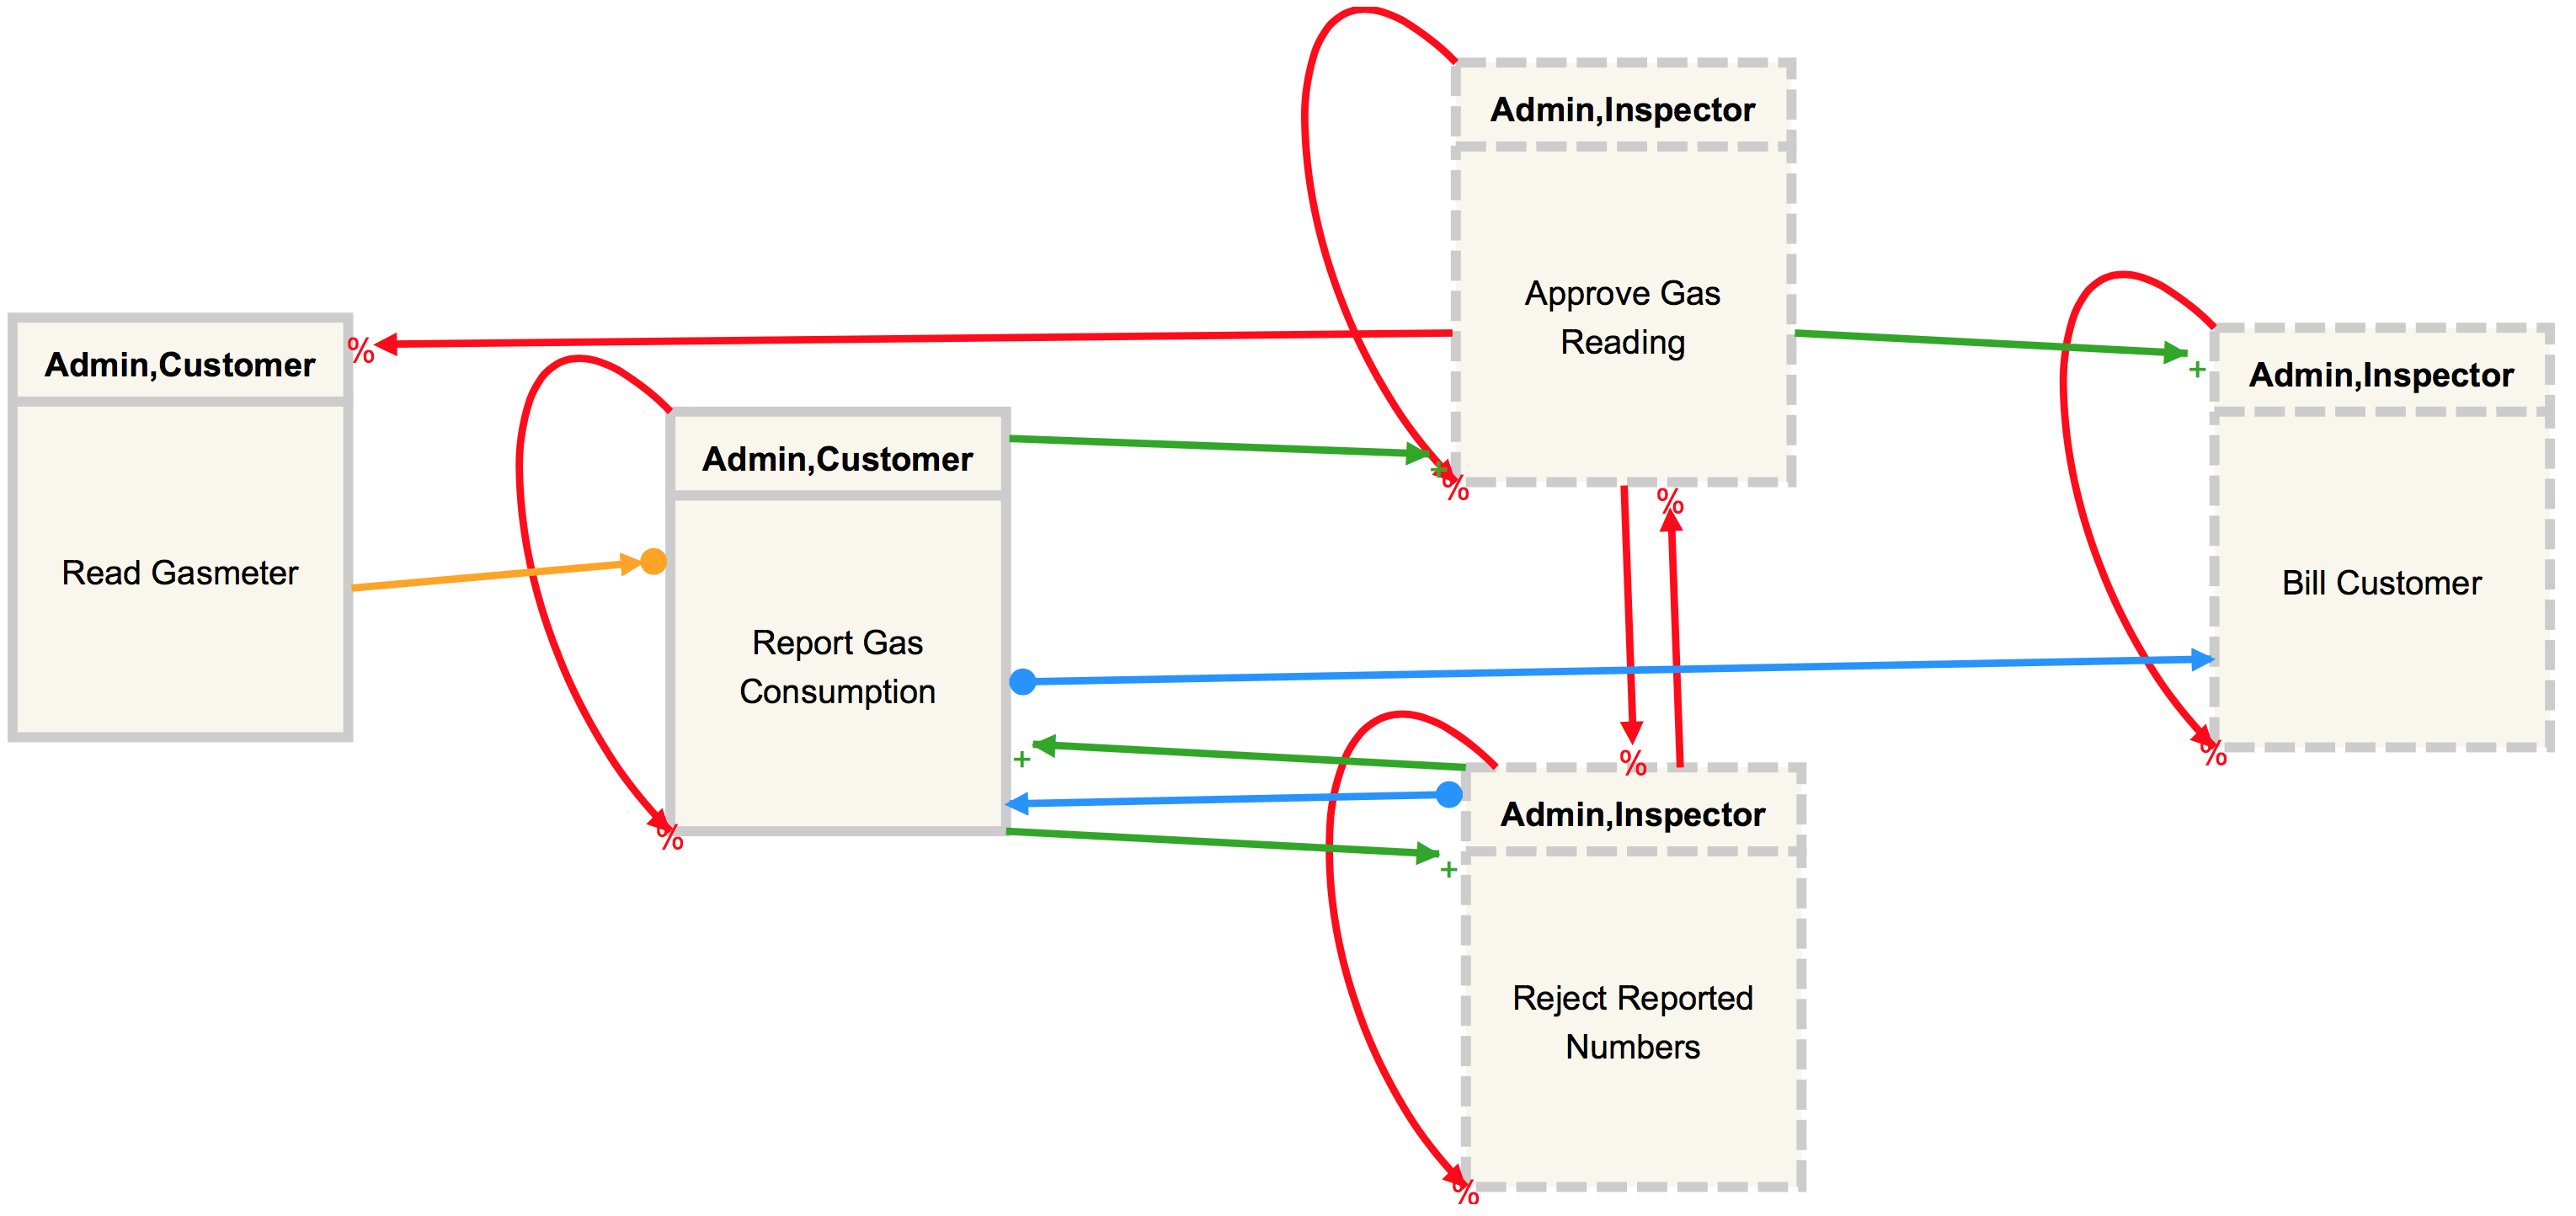
\includegraphics[width=\linewidth]{Figures/gas}
\caption{\label{SampleGasFlow} Sample Pay Yearly Gas Bill }
\end{figure}

A DCR graph represents a workflow. A workflow could, for instance, be the yearly reporting of gas consumption in a household, as seen in Figure \ref{SampleGasFlow}. A DCR graph is made up of a number of the following two components: \textit{events} and \textit{relations}. The term DCR \textit{graph} is due to events representing nodes, and relations representing edges between nodes.

\subsubsection{Events}
Events represent activities within a workflow. In the example, Figure \ref{SampleGasFlow}, there are five events, among others \textbf{Read Gasmeter} and \textbf{Bill Customer}. An event may have a role associated with it e.g. the event \textbf{Read Gasmeter} has a \textit{Customer}, and the event \textbf{Bill Customer} an \textit{Inspector}. The role determines who are allowed to execute the event. \\

A state for each event is needed for the functionality of a DCR graph to be implemented. The state of an event is comprised of the following information, see Table \ref{tab:TableOFDefaultValues} \\
\begin{table}[h!]
\centering
\begin{tabular}{|c|c|c|}\hline 
 & Options & Default value \\ \hline 
Pending & false $\vert$ true & false \\ \hline 
Included & false $\vert$ true & true \\ \hline
Executed & false $\vert$ true & false \\ \hline

\end{tabular} 
\caption{\label{tab:TableOFDefaultValues} Default values for event state}
\end{table}

\textit{Executed} describes if the event has been executed at least once. Depending on the value of \textit{Included} the event is either included: true, or excluded: false. \textit{Pending} describes if the event is expected to be executed eventually. For an event without relations to be executable the event must be included. After the execution of any event, their \textit{Pending} value must be set to false, and the \textit{Executed} value to true.

\subsubsection{Relations}
Relations describe constraints among events. There are 4 basic relations, explained in the following section. \\

\textbf{Condition - yellow arrow:} This relation states that to execute the event \textbf{B}, event \textbf{A} must be executed or excluded first. See Figure \ref{fig:ConditionRelation}.

\begin{figure}[H!]
\centering

\includegraphics[width=0.5\linewidth]{Figures/strawberry}
\caption{\label{fig:ConditionRelation} Illustration of Condition relation between event \textbf{A} and event \textbf{B}}
\end{figure} 

\textbf{Exclude - red arrow:} An exclusion relation states that once event \textbf{A} has been executed, the \textit{Included} boolean of event \textbf{B} must be set to false, such that event \textbf{B} is excluded. Note that an event may exclude itself, meaning once the event has executed, the \textit{Included} value of the event must be set to false such that it is excluded.  See figure \ref{fig:ExclusionRelation}.

\begin{figure}[H!]
\centering

\includegraphics[width=0.5\linewidth]{Figures/strawberry}
\caption{\label{fig:ExclusionRelation} Illustration of exclusion relation between event \textbf{A} and event \textbf{B}}
\end{figure} 


\textbf{Include - green arrow:} This relation states that event \textbf{A} includes event \textbf{B}. This means that  after the execution of event \textbf{A}, the \textit{Included} value of event \textbf{B} must be set to true, such that event \textbf{B} is included. See Figure \ref{fig:InclusionRelation}

\begin{figure}[H!]
\centering

\includegraphics[width=0.5\linewidth]{Figures/strawberry}
\caption{\label{fig:InclusionRelation} Illustration of inclusion relation between event \textbf{A} and event \textbf{B}}
\end{figure} 


\textbf{Response - blue arrow:} The response relation states that once event \textbf{A} is executed, event \textbf{B} is expected to be executed eventually. Once event \textbf{A} has been executed, the \textit{Pending} value of event \textbf{B} must be set to true. See Figure \ref{fig:ResponseRelation}

\begin{figure}[H!]
\centering

\includegraphics[width=0.5\linewidth]{Figures/strawberry}
\caption{\label{fig:ResponseRelation} Illustration of response relation between event \textbf{A} and event \textbf{B}}
\end{figure} 

To sum up: for an event to be executable, the \textit{Included} value must be true, and each of its condition relations must be either excluded or executed. \\

Furthermore an execution of an event leads to its \textit{Executed} and \textit{Pending} values to be set to true and false respectively. Each of the executed events’ response relations must have their \textit{Pending} value set to true, each of its inclusion relations must have their \textit{Included} value set to true, and its exclusion relations must have their \textit{Included} value set to false. \\

The three concepts: state, events, and relations, will be mirrored in the system.